\documentclass[../root.tex]{subfiles}

% Lengths for the matrix block plots
\newlength{\mycellheight}
\newlength{\innermargin}
\newlength{\cornerrad}
\newlength{\vsep}
\newlength{\msep}  % Offset from center
\newlength{\hsep}  % Offset between blocks
\newlength{\thirdlevelsep}

\newcommand{\white}[1]{{\color{white} #1}}
\newcommand{\0}{{\transparent{0} \resizebox{\mycellheight}{\mycellheight}{0}}}

\begin{document}

\chapter{A Parallel Linear System Solver for Optimal Control} \label{chap:rslqr}
\chaptermark{{rsLQR}}

\lettrine{E}{fficent} linear system solvers are a critical component of
numerical methods for solving optimal control problems.  Currently, most direct
methods for solving linear systems are serial, and only a few commercial
parallel direct methods exist.  We present a novel direct method that exploits
the sparse, banded structure that arises in optimal control problems, including
the prototypical LQR problem. Using a recursive application of Schur
complements, the algorithm has a theoretical $\mathcal{O}(\log(N))$ complexity
in the time horizon, and maps well onto many-core processors. An open-source
implementation demonstrates better performance than state-of-the-art commercial
parallel direct solvers designed for general sparse symmetric linear systems.

\section{Motivation} Parallel computing has changed many aspects of how we approach
algorithm development.  With single-processor speeds reaching asymptotic improvements, it
has become increasingly clear that substantial future improvements in computational
performance must come through parallelization, custom silicon, or often a combination of
both. While many algorithms in robotics are naturally parallelizable, especially the
data-driven approaches that frequently appear in perception and reinforcement learning, many
algorithms are still inherently serial and difficult to parallelize.  Numerous problems in robotics require solving large, sparse, and
nonlinearly-constrained optimization problems. Particularly in optimal control, these problems should 
ideally be solved online and onboard the robot, placing a high demand on computationally
efficient algorithms.

While some approaches to motion planning and control are naturally parallelizable, such as
sampling-based approaches like RRT \cite{lavalle_Rapidlyexploring_2001}, graph-based approaches that
rely on discretization of the configuration space \cite{lavalle_Planning_2006}, or
trajectory-sampling approaches like MPPI \cite{williams_Aggressive_2016}, they have many 
limitations. These algorithms often scale poorly with the dimension of the state space or
the time horizon, have limited ability to deal with complicated and/or underactuated
dynamics, or are limited by the types of constraints that can be imposed on the system, such
as those used to ensure either physically-realistic or safe state and control trajectories.
Optimization-based methods, on the other hand, offer many benefits over these approaches, 
and have received a lot of attention from both the academic and commercial robotics
communities over the past few years.

Typical approaches to optimal control and the related sub-problem of trajectory
optimization usually fall into one of two categories: DDP-based approaches that
rely on iteratively generating a local feedback law and simulating the system
forward under the closed-loop feedback policy
\cite{mayne_Secondorder_1966,tassa_Controllimited_2014,howell_ALTRO_2019,
jackson_ALTROC_2021,giftthaler_Family_2017,mastalli_Crocoddyl_2019,farshidian_Efficient_2017},
or direct collocation methods that solve the problem using general-purpose
nonlinear programming (NLP) solvers like SNOPT \cite{gill_SNOPT_2005}, Ipopt
\cite{wachter_Implementation_2006}, or Knitro
\cite{hargraves_Direct_1987,posa_Optimization_2016,betts_Practical_2001,hereid_FROST_2017, 
manchester_DIRTREL_2017,howell_Direct_2021}.
Both of these methods rely on forming a local approximation to the nonlinear
system, which requires 1st or 2nd-order Taylor series expansions of the cost,
dynamics, and constraints. The calculation of these expansions is trivially
parallelizable over the time horizon.  Parallelizing the optimization algorithm
itself, however, is much more challenging.

To parallelize DDP-based methods, the trajectory is split into many segments and ``glued''
back together by additional constraints
\cite{plancher_Performance_2020,farshidian_Realtime_2017, giftthaler_Family_2017}. While this
approach shows some promise, a recent study implementing DDP on a GPU found that increased
parallelism led to decreased convergence rates, leading to a natural limit to the amount of
parallelism that could be exploited \cite{plancher_Performance_2020}.  Direct methods, on the
other hand, are almost always dependent on general-purpose NLP solvers, all of which are
currently serial and single-threaded. The most computationally demanding part of these
algorithms is generally solving a large, sparse linear system of equations encoding the
local optimality conditions for the nonlinear optimization problem. Efficient methods for
parallelizing the solution of these linear systems are critical for unlocking the
computational improvements necessary to find trajectories for high-dimensional systems and
for long-horizon trajectories. 

This paper presents a novel method for solving the LQR problem, whose solution can be found 
by solving a banded linear system of equations. This linear system is prototypical of those 
found when solving optimal control problems with methods like sequential quadratic
programming (SQP). Using a hierarchical set of Schur complements inspired by the
nested-dissection algorithm used to solve problems for planar graphs
\cite{george_Nested_1973,khaira_Nested_}, we derive an algorithm with $\mathcal{O}(\log(N))$
complexity in the time horizon. With a modest amount of parallelism, this algorithm
outperforms the benchmark $\mathcal{O}(N)$ Riccati recursion that underlies DDP-based
algorithms, while being strictly more general in its applicability. We also show that the
algorithm is faster and scales better with increased parallelism than commercial parallel
linear-system solvers. Our algorithm is particularly well-suited to solving long-horizon
problems. The ability to efficiently handle long time horizons is often critical in
high-speed applications such as autonomous trucking, where a longer planning horizon has a
direct impact on the safety and performance of the controller. Even when solving problems
offline, such as finding low-thrust trajectories for space systems
\cite{tracy_LowThrust_2021}, reducing solve times from hours to minutes or seconds will have a
dramatic impact on the approaches we can take when searching for or designing such
trajectories. 

The remainder of this paper is structured as
follows: In Section \ref{sec:related_work} we survey methods for solving the LQR problem and
other related parallel solvers for optimal control. In Section \ref{sec:background} we 
review the linear quadratic regulator (LQR) problem and Schur complements. We derive our 
algorithm in Section \ref{sec:algorithm}, demonstrating a novel use of recursive
Schur complements to solve the LQR problem, followed by considerations for adapting the 
algorithm to work well on a many-core processor. The theoretical performance of the 
algorithm is compared to the Riccati solution in Section \ref{sec:results_theory}, which is 
followed up by a comparison of the actual open-source C implementation against
a suite of state-of-the-art sparse matrix solvers in Section \ref{sec:results_actual}, with 
concluding remarks in Section \ref{sec:rslqr_conclusion}.

\section{Related Work} \label{sec:related_work}
As one of the canonical problems in robotics, the LQR problem and its variants have received
a tremendous amount of attention over the past 60 years. The work most related to the
current one is a recent paper by Laine and Tomlin \cite{laine_Parallelizing_2019}, which
solves the LQR problem in parallel by splitting the trajectory into sub-trajectories and
adding additional constraints, based on previous work applying MPC to distributed systems
that used a nearly identical approach to decompose the distributed system into a set of
smaller problems \cite{soudbakhsh_Parallelized_2013}.

Recently, the traditional LQR problem has been extended to work with stage-wise
equality constraints \cite{brudigam_LinearTime_2020,yang_Equality_2020}. The linear
system \eqref{eq:qp_KKT} associated with LQR can also be solved using any of the
general techniques for solving sparse linear systems in parallel, including
parallel QR \cite{yang_Equality_2020}, block-cyclic reduction
\cite{hirshman_BCYCLIC_2010,gander_Cyclic_1997}, multigrid methods 
\cite{yang_BoomerAMG_2002,jones_Parallel_1997}, and indirect Krylov methods such as 
preconditioned conjugate-gradient \cite{anzt_Preconditioned_2017}.

Other notable work related to parallelizing optimal control or trajectory optimization problems
includes the qpDUNES solver \cite{frasch_Parallel_2015} that 
parallelizes over the time horizon using block-cyclic reduction, a recent paper solving 
contact-aware problems on a GPU using a combination of indirect methods and block-cyclic 
reduction \cite{pan_GPUbased_2019}, an FPGA implementation of a linear MPC solver using the 
MINRES indirect method \cite{jerez_Parallel_2011}, and a variety of ADMM or augmented 
Lagrangian-based methods \cite{kouzoupis_Block_2016, yu_Efficient_2017,alonso_Effective_2021,
zhou_Accelerated_2020,sindhwani_Sequential_2017}.

Like \cite{laine_Parallelizing_2019}, the proposed algorithm parallelizes the LQR problem over
the time horizon, but instead of assuming an explicit discrete dynamics function, our 
algorithm can be trivially extended to work with implicit integrators such as the 
Hermite-Simpson method commonly found when solving optimal control problems with direct 
collocation. It can also easily handle stage-wise equality constraints. 

While the proposed algorithm borrows ideas from the literature on solving symmetric sparse
linear systems in parallel, it is, to the authors' best knowledge, a novel application and
specialization of those ideas to the optimal control problem. We also provide a documented 
open-source parallelized implementation of our algorithm with a convenient wrapper written
in a high-level programming language, where many of the previously cited works are purely 
theoretical or don't provide an open-source implementation.

\section{Background} \label{sec:background}
\subsection{Notation}
We use interval notation $j \in (a,b] := \{a+1,a+2,\dots,b\}$, $j \in [a,b] :=
\{a,a+1,\dots,b\}$, for $j,a,b \in \mathbb{N}$ to denote sets of consecutive integers. 
We use angle-bracket notation $\langle x, y \rangle$ to denote $x^T y$ for both 
vectors and matrix arguments. 

\subsection{The Linear Quadratic Regulator}
The Linear Quadratic Regulator (LQR) problem is the canonical problem in optimal control, 
since it can be solved using a variety of methods and is amenable to theoretical analysis. It 
is also of practical significance since LQR problems arise when an unconstrained nonlinear 
optimal control problem is approximated using a 2nd-order Taylor expansion of the cost 
function and a linear approximation of the dynamics. The LQR problem, shown here with 
affine terms included, has the form:
\begin{mini}[2]
    {x_{1:N}, u_{1:N-1}}{ 
        \sum_{k=1}^{N} \half x_k^T Q_k x_k + q_k^T x_k \hspace{0em}}{}{}
    \breakObjective{+ \sum_{k=1}^{N-1} \half u_k^T R_k u_k + r_k^T u_k}
    \addConstraint{x_{k+1} = \hat{A}_k x_k + \hat{B}_k u_k + f_k = 0 }
    \addConstraint{x_1 = x_\text{init}} 
    \label{opt:qp}
\end{mini}
where $x_k \in \R^n$ and $u_k \in \R^m$ are the state and control vectors at time step $k$,
$N$ is the number of time steps (also referred to as the time horizon),
and $\hat{A} \in \R^{n \times n}, \hat{B} \in \R^{n \times m}, f \in \R^n, Q \in 
\R^{n \times n}, R \in \R^{m \times m}, q \in \R^n$, and $r \in \R^m$ come from the 
Taylor expansions of the cost and dynamics about some reference trajectory (or point).

The well-known first-order optimality, or KKT, conditions for \eqref{opt:qp} are 
\cite{boyd_Convex_2004}:
\begin{subequations}
\begin{align}
    &Q_k x_k + q_k + \hat{A}_k^T \lambda_{k+1} - \lambda_k = 0, \quad k \in [1,N) \\
    &R_k u_k + r_k + \hat{B}_k^T \lambda_{k+1} = 0, \quad k \in [1,N) \\
    &Q_N x_N + q_N - \lambda_N = 0  \\
    &x_{k+1} = \hat{A}_k x_k + \hat{B}_k u_k + f_k, \; k \in [1,N) \\
    &x_1 = x_\text{init}
\end{align}
\end{subequations}
which can be written in matrix form as the following linear system:
\begin{equation} \label{eq:linear_system}
    H v = g
\end{equation}
where for $N$ = 4:
{
\setlength\arraycolsep{1pt}
\renewcommand{\arraystretch}{0.8}
\begin{subequations}
\begin{align} \label{eq:qp_KKT}
    H &= \scalebox{1.0}{$
    \begin{bmatrix}
         Q_1 &&&&&&& -I & \hat{A}_1^T \\
        & R_1 &&&&&&    & \hat{B}_1^T \\
        && Q_2 &&&&&    & -I          & \hat{A}_2^T \\
        &&& R_2 &&&&    &             & \hat{B}_2^T \\
        &&&& Q_3 &&&    &             & -I & \hat{A} \\
        &&&&& R_3 &&    &             &    & \hat{B} \\
        &&&&&& Q_4 &    &             &    & -I \\
        -I \\
        \hat{A}_1 & \hat{B}_1 & -I &   \\
        && \hat{A}_2 & \hat{B}_2 & -I \\
        &&&& \hat{A}_3 & \hat{B}_3 & -I \\
    \end{bmatrix}
    $} \\
    v &= \begin{bmatrix}
        x_1^T & u_1^T & x_2^T & u_2^T & x_3^T & u_3^T & x_4^T & \lambda_1^T & \lambda_2^T & \lambda_3^T & \lambda_4^T
    \end{bmatrix}^T \\
    g &= -\begin{bmatrix}
        q_1^T & r_1^T & q_2^T & r_2^T & q_3^T & r_3^T & q_4^T & x_\text{init}^T & f_1^T & f_2^T & f_3^T
    \end{bmatrix}^T
\end{align}
\end{subequations}
}
\noindent Note that $H$ is a symmetric, quasidefinite matrix (known as a KKT matrix) with $Nn + (N-1)m$ positive 
eigenvalues and $Nn$ negative eigenvalues \cite{boyd_Convex_2004}.

\subsection{Schur complements} \label{sec:schur_complements}
A Schur complement is a common trick that reduces solving a single large linear system to solving a 
series of smaller ones. We will use the
Schur complement to solve symmetric 3x3 block-tridiagonal systems of the form: 
\begin{equation} \label{eq:schur_3x3}
    \begin{bmatrix}
        A   & D & \\
        D^T & B & E^T \\
            & E & C \\
    \end{bmatrix}
    \begin{bmatrix}
        x \\ y \\ z
    \end{bmatrix} = 
    \begin{bmatrix}
        a \\ b \\ c
    \end{bmatrix}.
\end{equation}
We can solve the first and last rows of \eqref{eq:schur_3x3} for $x$ and $z$:
\begin{subequations} \label{eq:schur_xz}
\begin{align}
    &x = A^{-1}(a - D y) = \bar{a} - \bar{D} y \label{eq:schur_x}, \\
    &z = C^{-1}(c - E y) = \bar{c} - \bar{E} y \label{eq:schur_z},
\end{align}
\end{subequations}
where we calculate the following pieces numerically by factorizing $A$ and $C$:
\begin{subequations} \label{eq:schur_temps}
\begin{align}
    &\bar{D} = A^{-1} D, \quad \bar{a} = A^{-1} a, \\
    &\bar{E} = C^{-1} E, \quad \bar{c} = C^{-1} c.
\end{align}
\end{subequations}
We can use \eqref{eq:schur_xz} to eliminate $x$ and $z$ from the middle row, allowing us to 
solve for $y$:
\begin{equation} \label{eq:schur_y}
    \begin{aligned}
        y &= -(D^T \bar{D} + E^T \bar{E} - B)^{-1}(b - E^T \bar{c} - D^T \bar{a}) \\
          &= -\bar{B}^{-1} \bar{b}
    \end{aligned}
\end{equation}
After solving \eqref{eq:schur_y} numerically, we can now plug the result into
\eqref{eq:schur_xz} to get our completed solution vector. 


\begin{figure}[t!]
    \centering
    \begin{equation}
        \renewcommand{\arraystretch}{0.8}
        \setlength\arraycolsep{1pt}
        \resizebox{\columnwidth-4.0em}{!}{$
        \begin{bNiceMatrix}
        \Block[fill=red!40!white, rounded-corners=4pt]{5-5}{}
        Q_1       &           & \hat{A}_1^T &           &           & \Block[fill=green!40!white, rounded-corners=4pt]{5-1}{} \\
                  & R_1       & \hat{B}_1^T \\
        \hat{A}_1 & \hat{B}_1 &             & -I \\
                  &           & -I          & Q_2       &           & \hat{A}_2^T \\
                  &           &             &           & R_2       & \hat{B}_2^T \\
            \Block[fill=green!40!white, rounded-corners=4pt]{1-5}{}
                  &           &             & \hat{A}_2 & \hat{B}_2 & \Block[fill=green!40!white, rounded-corners=4pt]{1-1}{}
                                                        & \Block[fill=green!40!white, rounded-corners=4pt]{1-5}{}
                                                          -I \\
                  &           &             &           &           & \Block[fill=green!40!white, rounded-corners=4pt]{5-1}{}
                                        -I    & \Block[fill=red!40!white, rounded-corners=4pt]{5-5}{}
                                                Q_3 &     & \hat{A}_3^T \\
            &     &       &     &     &       &     & R_3 & \hat{B}_3^T \\
            &     &       &     &     &       & \hat{A}_3 & \hat{B}_3 &       & -I \\
            &     &       &     &     &       &     &     & -I    & Q_4 &     \\
            &     &       &     &     &       &     &     &       &     & R_3 \\
        \end{bNiceMatrix}
        \begin{bNiceMatrix}
        \Block[fill=blue!40!white, rounded-corners]{5-1}{}
        x_1 \\ u_1 \\ \lambda_2 \\ x_2 \\ u_2 \\ 
        \Block[fill=green!40!white, rounded-corners]{1-1}{}
        \lambda_3 \\ 
        \Block[fill=blue!40!white, rounded-corners=4pt]{5-1}{}
        x_3 \\ u_3 \\ \lambda_4 \\ x_4 \\ u_4
        \end{bNiceMatrix}
        =
        -\begin{bNiceMatrix}
        \Block[fill=blue!40!white, rounded-corners]{5-1}{}
        q_1 \\ r_1 \\ f_1 \\ q_2 \\ r_2 \\ 
        \Block[fill=green!40!white, rounded-corners]{1-1}{}
        f_2 \\ 
        \Block[fill=blue!40!white, rounded-corners]{5-1}{}
        q_3 \\ r_3 \\ f_3 \\ q_4 \\ r_4
        \end{bNiceMatrix}
        $}
    \end{equation}
    \caption{
        The LQR linear system, rearranged and partitioned to appear in the form of
        \eqref{eq:schur_3x3}. The red block in the upper left corner is $A$, the red
        lower-right block is $C$.  The top vertical green block is $D$, and the bottom
        green vertical block is $E$. The solution and right-hand-side vectors have also been 
        partitioned, with the top blue blocks equating to $x$ and $a$, the middle green 
        block to $y$ and $b$, and the bottom blue blocks to $z$ and $c$. 
        We use these blocks to solve the LQR problem using the steps
        in Sec. \ref{sec:schur_complements}.
    }
    \label{fig:kkt_schur}
\end{figure}



\section{A Parallel LQR Algorithm} \label{sec:algorithm}

\subsection{Recursive Schur complements}
We now derive our parallelizable algorithm for solving linear systems of the form 
\eqref{eq:linear_system}. First, we reorder the rows and columns of \eqref{eq:qp_KKT}
to get a banded matrix with a bandwidth of $2n + m -1$ (see Fig. \ref{fig:kkt_schur}).


Note that, for clarity, we've ignored the special boundary conditions at the first and last 
time steps. From the coloring we see that the LQR problem takes the 3x3 block tridiagonal 
form of \eqref{eq:schur_3x3}. When solving for $\bar{a}, \bar{c}, \bar{D}$, and $\bar{E}$ 
in \eqref{eq:schur_temps} we make a critical observation:
\begin{subequations} \label{eq:level_1}
\begin{align}
    \resizebox{\columnwidth-3.5em}{!}{
    \renewcommand{\arraystretch}{0.9}
    \setlength\arraycolsep{1pt}
    $
    \begin{NiceMatrix}
        \Block[fill=green!40!white, rounded-corners]{5-1}{\makebox[1em][c]{$\bar{D}$}} \\ \\ \\ \\ \\
    \end{NiceMatrix} =
    -\begin{bNiceMatrix}
    \Block[fill=orange!40!white, rounded-corners=4pt]{2-2}{}
        \Block[fill=orange!40!white, rounded-corners=4pt]{2-2}{}
        Q_1 &     & \Block[fill=red!40!white, rounded-corners=4pt]{2-1}{}
                    \hat{A}_1^T &     &     \\
            & R_1 & \hat{B}_1^T \\
        \Block[fill=red!40!white, rounded-corners]{1-2}{}
        \hat{A}_1 & \hat{B}_1 & \Block[fill=red!40!white, rounded-corners]{1-1}{}
                        & \Block[fill=red!40!white, rounded-corners]{1-2}{}
                            -I \\
            &     & \Block[fill=red!40!white, rounded-corners]{2-1}{}
                    -I    & \Block[fill=orange!40!white, rounded-corners]{2-2}{}
                            Q_2 &     \\
            &     &       &     & R_2 \\
    \end{bNiceMatrix} ^{-1}
    \begin{bNiceMatrix}
        \Block[fill=green!40!white, rounded-corners]{2-1}{} \\ \\ 
        \Block[fill=red!40!white, rounded-corners]{1-1}{} \\ 
        \Block[fill=green!40!white, rounded-corners]{2-1}{} A_2^T \\ B_2^T \\ 
    \end{bNiceMatrix}, \;
    \begin{NiceMatrix}
        \Block[fill=blue!40!white, rounded-corners]{5-1}{\makebox[1em][c]{$\bar{a}$}} \\ \\ \\ \\ \\
    \end{NiceMatrix} =
    -\begin{bNiceMatrix}
        \Block[fill=orange!40!white, rounded-corners=4pt]{2-2}{}
        Q_1 &     & \Block[fill=red!40!white, rounded-corners=4pt]{2-1}{}
                    \hat{A}_1^T &     &     \\
            & R_1 & \hat{B}_1^T \\
        \Block[fill=red!40!white, rounded-corners]{1-2}{}
        \hat{A}_1 & \hat{B}_1 & \Block[fill=red!40!white, rounded-corners]{1-1}{}
                        & \Block[fill=red!40!white, rounded-corners]{1-2}{}
                            -I \\
            &     & \Block[fill=red!40!white, rounded-corners]{2-1}{}
                    -I    & \Block[fill=orange!40!white, rounded-corners]{2-2}{}
                            Q_2 &     \\
            &     &       &     & R_2 \\
    \end{bNiceMatrix} ^{-1}
    \begin{bNiceMatrix}
        \Block[fill=blue!40!white, rounded-corners]{2-1}{}
        q_1 \\ r_1 \\ 
        \Block[fill=red!40!white, rounded-corners]{1-1}{}
        f_1 \\ 
        \Block[fill=blue!40!white, rounded-corners]{2-1}{}
        q_2 \\ r_2 \\ 
    \end{bNiceMatrix}, \;
    $} \label{eq:level_1_1} \\
    %
    \resizebox{\columnwidth-3.5em}{!}{
    \renewcommand{\arraystretch}{0.9}
    \setlength\arraycolsep{1pt}
    $
    \begin{NiceMatrix}
        \Block[fill=green!40!white, rounded-corners]{5-1}{\makebox[1em][c]{$\bar{E}$}} \\ \\ \\ \\ \\
    \end{NiceMatrix} =
    -\begin{bNiceMatrix}
        \Block[fill=orange!40!white, rounded-corners=4pt]{2-2}{}
        Q_3 &     & \Block[fill=red!40!white, rounded-corners=4pt]{2-1}{}
                    \hat{A}_3^T &     &     \\
            & R_3 & \hat{B}_3^T \\
        \Block[fill=red!40!white, rounded-corners]{1-2}{}
        \hat{A}_3 & \hat{B}_3 & \Block[fill=red!40!white, rounded-corners]{1-1}{}
                        & \Block[fill=red!40!white, rounded-corners]{1-2}{}
                            -I \\
            &     & \Block[fill=red!40!white, rounded-corners]{2-1}{}
                    -I    & \Block[fill=orange!40!white, rounded-corners]{2-2}{}
                            Q_4 &     \\
            &     &       &     & R_4 \\
    \end{bNiceMatrix} ^{-1}
    \begin{bNiceMatrix}
        \Block[fill=green!40!white, rounded-corners]{2-1}{} -I \\ \\ 
        \Block[fill=red!40!white, rounded-corners]{1-1}{} \\ 
        \Block[fill=green!40!white, rounded-corners]{2-1}{} \\ \\ 
    \end{bNiceMatrix}, \;
    \begin{NiceMatrix}
        \Block[fill=blue!40!white, rounded-corners]{5-1}{\makebox[1em][c]{$\bar{c}$}} \\ \\ \\ \\ \\
    \end{NiceMatrix} =
    -\begin{bNiceMatrix}
        \Block[fill=orange!40!white, rounded-corners=4pt]{2-2}{}
        Q_3 &     & \Block[fill=red!40!white, rounded-corners=4pt]{2-1}{}
                    \hat{A}_3^T &     &     \\
            & R_3 & \hat{B}_3^T \\
        \Block[fill=red!40!white, rounded-corners]{1-2}{}
        \hat{A}_3 & \hat{B}_3 & \Block[fill=red!40!white, rounded-corners]{1-1}{}
                        & \Block[fill=red!40!white, rounded-corners]{1-2}{}
                            -I \\
            &     & \Block[fill=red!40!white, rounded-corners]{2-1}{}
                    -I    & \Block[fill=orange!40!white, rounded-corners]{2-2}{}
                            Q_4 &     \\
            &     &       &     & R_4 \\
    \end{bNiceMatrix} ^{-1}
    \begin{bNiceMatrix}
        \Block[fill=blue!40!white, rounded-corners]{2-1}{}
        q_3 \\ r_3 \\ 
        \Block[fill=red!40!white, rounded-corners]{1-1}{}
        f_3 \\ 
        \Block[fill=blue!40!white, rounded-corners]{2-1}{}
        q_4 \\ r_4 \\ 
    \end{bNiceMatrix}. \;
    $} \label{eq:level_1_2}
\end{align}
\end{subequations}
Due to the banded structure of the matrix, each of these smaller linear systems also takes the 
form of \eqref{eq:schur_3x3}. Note that, for each diagonal $A$ or $C$ block, we solve two 
linear systems, one with right-hand-side data from the original right-hand-side vector 
(shown in blue), and one with right-hand-side data from the green columns in Fig.
\ref{fig:kkt_schur}.

If we apply the same technique to each of these 4 linear systems, we'd get 16 total linear
systems to solve. However, after eliminating duplicates, we're left with 12 unique small linear 
systems,
\begin{subequations} \label{eq:level_2}
\begin{align}
    \resizebox{\columnwidth-4.5em}{!}{
        \renewcommand{\arraystretch}{0.9}
        \setlength\arraycolsep{1pt}
        $
        \begin{NiceMatrix}
            \Block[fill=red!40!white, rounded-corners]{2-1}{\makebox[1em]{$\bar{D}_1$}} \\ \\
        \end{NiceMatrix}^{(1)} \hspace{-0.5em} = 
        -\begin{bNiceMatrix}
            \Block[fill=orange!40!white, rounded-corners]{2-2}{} Q_1 \\ & R_1 \\
        \end{bNiceMatrix}^{-1}
        \begin{bNiceMatrix}
            \Block[fill=red!40!white, rounded-corners]{2-1}{}
            \hat{A}_1^T \\ \hat{B}_1^1 \\
        \end{bNiceMatrix}, \;
        \begin{NiceMatrix}
            \Block[fill=green!40!white, rounded-corners]{2-1}{\makebox[1em]{$\bar{a}_1$}} \\ \\
        \end{NiceMatrix}^{(1,2)} \hspace{-1.2em} =
        -\begin{bNiceMatrix}
            \Block[fill=orange!40!white, rounded-corners]{2-2}{} Q_1 \\ & R_1 \\
        \end{bNiceMatrix}^{-1}
        \begin{bNiceMatrix}
            \Block[fill=green!40!white, rounded-corners]{2-1}{}
            \makebox[1.5em]{$0$} \\ 0 \\
        \end{bNiceMatrix}, \;
        \begin{NiceMatrix}
            \Block[fill=blue!40!white, rounded-corners]{2-1}{\makebox[1em]{$\bar{a}_1$}} \\ \\
        \end{NiceMatrix}^{(1,3)} \hspace{-1.2em} =
        -\begin{bNiceMatrix}
            \Block[fill=orange!40!white, rounded-corners]{2-2}{} Q_1 \\ & R_1 \\
        \end{bNiceMatrix}^{-1}
        \begin{bNiceMatrix}
            \Block[fill=blue!40!white, rounded-corners]{2-1}{}
            q_1 \\ r_1 \\
        \end{bNiceMatrix}, \;
    $} \label{eq:level_2_1} \\
    %
    \resizebox{\columnwidth-4.5em}{!}{
        \renewcommand{\arraystretch}{0.9}
        \setlength\arraycolsep{1pt}
        $
        \begin{NiceMatrix}
            \Block[fill=red!40!white, rounded-corners]{2-1}{\makebox[1em]{$\bar{E}_1$}} \\ \\
        \end{NiceMatrix}^{(1)} \hspace{-0.5em} = 
        -\begin{bNiceMatrix}
            \Block[fill=orange!40!white, rounded-corners]{2-2}{} Q_2 \\ & R_2 \\
        \end{bNiceMatrix}^{-1}
        \begin{bNiceMatrix}
            \Block[fill=red!40!white, rounded-corners]{2-1}{}
            -I \\ \\
        \end{bNiceMatrix}, \;
        \begin{NiceMatrix}
            \Block[fill=green!40!white, rounded-corners]{2-1}{\makebox[1em]{$\bar{c}_1$}} \\ \\
        \end{NiceMatrix}^{(1,2)} \hspace{-1.2em} = 
        -\begin{bNiceMatrix}
            \Block[fill=orange!40!white, rounded-corners]{2-2}{} Q_2 \\ & R_2 \\
        \end{bNiceMatrix}^{-1}
        \begin{bNiceMatrix}
            \Block[fill=green!40!white, rounded-corners]{2-1}{}
            \hat{A}_2^T \\ \hat{B}_2^T \\
        \end{bNiceMatrix}, \;
        \begin{NiceMatrix}
            \Block[fill=blue!40!white, rounded-corners]{2-1}{\makebox[1em]{$\bar{c}_1$}} \\ \\
        \end{NiceMatrix}^{(1,3)} \hspace{-1.2em} = 
        -\begin{bNiceMatrix}
            \Block[fill=orange!40!white, rounded-corners]{2-2}{} Q_2 \\ & R_2 \\
        \end{bNiceMatrix}^{-1}
        \begin{bNiceMatrix}
            \Block[fill=blue!40!white, rounded-corners]{2-1}{}
            q_2 \\ r_2 \\
        \end{bNiceMatrix}, \;
    $} \label{eq:level_2_2} \\
    \resizebox{\columnwidth-4.5em}{!}{
        \renewcommand{\arraystretch}{0.9}
        \setlength\arraycolsep{1pt}
        $
        \begin{NiceMatrix}
            \Block[fill=red!40!white, rounded-corners]{2-1}{\makebox[1em]{$\bar{D}_2$}} \\ \\
        \end{NiceMatrix}^{(1)} \hspace{-0.5em} = 
        -\begin{bNiceMatrix}
            \Block[fill=orange!40!white, rounded-corners]{2-2}{} Q_3 \\ & R_3 \\
        \end{bNiceMatrix}^{-1}
        \begin{bNiceMatrix}
            \Block[fill=red!40!white, rounded-corners]{2-1}{}
            \hat{A}_3^T \\ \hat{B}_3^1 \\
        \end{bNiceMatrix}, \;
        \begin{NiceMatrix}
            \Block[fill=green!40!white, rounded-corners]{2-1}{\makebox[1em]{$\bar{a}_2$}} \\ \\
        \end{NiceMatrix}^{(1,2)} \hspace{-1.2em} = 
        -\begin{bNiceMatrix}
            \Block[fill=orange!40!white, rounded-corners]{2-2}{} Q_3 \\ & R_3 \\
        \end{bNiceMatrix}^{-1}
        \begin{bNiceMatrix}
            \Block[fill=green!40!white, rounded-corners]{2-1}{}
            -I \\ \\
        \end{bNiceMatrix}, \;
        \begin{NiceMatrix}
            \Block[fill=blue!40!white, rounded-corners]{2-1}{\makebox[1em]{$\bar{a}_2$}} \\ \\
        \end{NiceMatrix}^{(1,3)} \hspace{-1.2em} = 
        -\begin{bNiceMatrix}
            \Block[fill=orange!40!white, rounded-corners]{2-2}{} Q_3 \\ & R_3 \\
        \end{bNiceMatrix}^{-1}
        \begin{bNiceMatrix}
            \Block[fill=blue!40!white, rounded-corners]{2-1}{}
            q_3 \\ r_3 \\
        \end{bNiceMatrix}, \;
    $} \label{eq:level_2_3} \\
    %
    \resizebox{\columnwidth-4.5em}{!}{
        \renewcommand{\arraystretch}{0.9}
        \setlength\arraycolsep{1pt}
        $
        \begin{NiceMatrix}
            \Block[fill=red!40!white, rounded-corners]{2-1}{\makebox[1em]{$\bar{E}_2$}} \\ \\
        \end{NiceMatrix}^{(1)} \hspace{-0.5em} = 
        -\begin{bNiceMatrix}
            \Block[fill=orange!40!white, rounded-corners]{2-2}{} Q_4 \\ & R_4 \\
        \end{bNiceMatrix}^{-1}
        \begin{bNiceMatrix}
            \Block[fill=red!40!white, rounded-corners]{2-1}{}
            -I \\ \\
        \end{bNiceMatrix}, \;
        \begin{NiceMatrix}
            \Block[fill=green!40!white, rounded-corners]{2-1}{\makebox[1em]{$\bar{c}_2$}} \\ \\
        \end{NiceMatrix}^{(1,2)} \hspace{-1.2em} = 
        -\begin{bNiceMatrix}
            \Block[fill=orange!40!white, rounded-corners]{2-2}{} Q_4 \\ & R_4 \\
        \end{bNiceMatrix}^{-1}
        \begin{bNiceMatrix}
            \Block[fill=green!40!white, rounded-corners]{2-1}{}
            \makebox[1.5em]{$0$} \\ 0 \\
        \end{bNiceMatrix}, \;
        \begin{NiceMatrix}
            \Block[fill=blue!40!white, rounded-corners]{2-1}{\makebox[1em]{$\bar{c}_2$}} \\ \\
        \end{NiceMatrix}^{(1,3)} \hspace{-1.2em} = 
        -\begin{bNiceMatrix}
            \Block[fill=orange!40!white, rounded-corners]{2-2}{} Q_4 \\ & R_4 \\
        \end{bNiceMatrix}^{-1}
        \begin{bNiceMatrix}
            \Block[fill=blue!40!white, rounded-corners]{2-1}{}
            q_4 \\ r_4 \\
        \end{bNiceMatrix}, \;
    $} \label{eq:level_2_4} 
\end{align}
\end{subequations}
where \eqref{eq:level_2_1} and \eqref{eq:level_2_2} come from \eqref{eq:level_1_1} and
\eqref{eq:level_2_3} and \eqref{eq:level_2_4} come from \eqref{eq:level_1_2}.  We also
introduce some notation, since we need to distinguish between all of the different $\bar{a},
\bar{c}, \bar{D},$ and $\bar{E}$ blocks. We use $\bar{a}_i^{(j,p)}$ and $\bar{c}_i^{(j,p)}$
to denote the $i$th $\bar{a}$ or $\bar{c}$ at a recursion depth of $j$ using right-hand-side
data from a ``parent'' depth of $p$, where depth is measured from the bottom. We also note
that, as suggested by \eqref{eq:level_2}, $\bar{a}_i^{(j,j)} = \bar{D}_i^{(j)}$ and
$\bar{c}_i^{(j,j)} = \bar{E}_i^{(j)}$. The notation is further clarified in Fig.
\ref{fig:kkt_partitioned}. Since the linear systems in \eqref{eq:level_1} all involve 
block-diagonal matrices, we can solve all of these systems directly using e.g. a dense
Cholesky decomposition.  With these pieces we use \eqref{eq:schur_y} to get all the $y$'s,
followed by \eqref{eq:schur_xz} to get all the $x$'s and $z$'s, which concatentated form the
$\bar{a}$, $\bar{c}$, $\bar{D}$, and $\bar{E}$ at the next level, i.e. \eqref{eq:level_1}.
These are then used to solve the top-level Schur complement for the solution vector using
the same procedure.

\newcommand{\SP}{\makebox[1em]{}}
% \newcommand{\SP}{\parbox[c][1em][c]{1em}{}}
\begin{figure}
    \begin{equation*} \label{eq:kkt_partitioned}
        \renewcommand{\arraystretch}{1.0}
        \setlength\arraycolsep{1pt}
        \resizebox{\columnwidth-3.0em}{!}{$
        H = \begin{bNiceMatrix}
        \Block[fill=orange!40!white, rounded-corners=4pt]{2-2}{A_1^{(1)}}
        \SP &     & \Block[fill=red!40!white, rounded-corners]{2-1}{D_1^{(1)}}
                          &     &     & \Block[fill=green!40!white, rounded-corners=4pt]{5-1}{D_1^{(2)}} \\
            & \SP &       \\
        \Block[fill=red!40!white, rounded-corners]{1-2}{}
        \SP & \SP & \Block[fill=red!40!white, rounded-corners]{1-1}{B_1^{(1)}} 
                          & \Block[fill=red!40!white, rounded-corners]{1-2}{}
                               \\
            &     & \Block[fill=red!40!white, rounded-corners]{2-1}{E_1^{(1)}}
                          & \Block[fill=orange!40!white, rounded-corners]{2-2}{C_1^{(1)}}
                            \SP &     &       \\
            &     &       &     & \SP &       \\
            \Block[fill=green!40!white, rounded-corners=4pt]{1-5}{}
            &     &       & \SP & \SP & \Block[fill=green!40!white, rounded-corners=4pt]{1-1}{B_1^{(2)}}
                                            & \Block[fill=green!40!white, rounded-corners=4pt]{1-5}{}
                                                   \\
            &     &       &     &     & \Block[fill=green!40!white, rounded-corners=4pt]{5-1}{E_1^{(2)}}
                                         \SP  & \Block[fill=orange!40!white, rounded-corners=4pt]{2-2}{A_2^{(1)}} \Block[draw=black, rounded-corners]{5-5}{}
                                                \SP &     & \Block[fill=red!40!white, rounded-corners=4pt]{2-1}{D_2^{(1)}}
                                                                  \\
            &     &       &     &     &       &     & \SP &       \\
            &     &       &     &     &       & \Block[fill=red!40!white, rounded-corners=4pt]{1-2}{}
                                                \SP & \SP & \Block[fill=red!40!white, rounded-corners]{1-1}{B_2^{(1)}}
                                                                  & \Block[fill=red!40!white, rounded-corners=4pt]{1-2}{} \\
            &     &       &     &     & \Block[draw=red,rounded-corners]{2-1}{}
                                                    &     &     & \Block[fill=red!40!white, rounded-corners=4pt]{2-1}{E_2^{(1)}}
                                                                  & \Block[fill=orange!40!white, rounded-corners=4pt]{2-2}{C_2^{(1)}}
                                                                    \SP &     \\
            &     &       &     &     &       &     &     &       &     & \SP \\
        \end{bNiceMatrix}, \;
        g =
        \begin{bNiceMatrix}
        \Block[fill=blue!40!white, rounded-corners]{2-1}{a_1^{(1,3)}}
        \SP \\ \SP \\ 
        \Block[fill=red!40!white, rounded-corners]{1-1}{b_1^{(1,3)}}
        \SP \\ 
        \Block[fill=blue!40!white, rounded-corners]{2-1}{c_1^{(1,3)}}
        \SP \\ \SP \\ 
        \Block[fill=green!40!white, rounded-corners]{1-1}{b_1^{(2,3)}}
        \SP \\ 
        \Block[fill=blue!40!white, rounded-corners]{2-1}{a_2^{(1,3)}}
        \SP \\ \SP \\ 
        \Block[fill=red!40!white, rounded-corners]{1-1}{b_2^{(1,3)}}
        \SP \\ 
        \Block[fill=blue!40!white, rounded-corners]{2-1}{c_2^{(1,3)}}
        \SP \\ \SP
        \end{bNiceMatrix}
        $}
    \end{equation*}
    \caption{The LQR KKT system after recursively partitioning with Schur complements with a 
        depth of $K=2 = \log_2(N)$ with $N=4$. The labels follow the notation used in
        Algorithm \ref{alg:recursive_schur}. Levels are enumerated starting at $j=1$ for the
        deepest recursion level (the orange and red blocks), up to $j=K$ (the green blocks).
        We assign the right-hand-side vector a level of $K+1$ (the blue blocks). We use
        $A_i^{(j)}$ and $C_i^{(j)}$ to denote the $i$th $A$ and $C$ blocks at level $j$,
        e.g.  the block outlined in black is $C_1^{(2)}$. We use the same notation for
        $D_i^{(j)}$ and $E_i^{(j)}$, as shown. We use $a_i^{(j,p)}$ and $c_i^{(j,p)}$ to
        refer to the block with the rows of $D_i^{(j)}$ and $E_i^{(j)}$, respectively, and
        the columns of either $D_i^{(p)}$ or $E_i^{(p)}$. For example, the block outlined in
        red is $c_2^{(1,2)}$ since it corresponds to the rows of the red block $E_2^{(1)}$
        but taken from the green data / columns of level $p=2$. Since the right-hand-side
        vector $g$ is given a level of $K+1$, its blocks all have $p=3$. We've partitioned
        the $g$ vector from the lowest level, coloring the blocks corresponding to the
        $B_i^{(j)}$ blocks to match the level $j$.
    }
    \label{fig:kkt_partitioned}
\end{figure}
It should be clear that the resulting algorithm is naturally recursive and results in a
binary tree of Schur complements, since each 3x3 Schur complement requires solving another
Schur complement problem for both $A$ and $C$. Borrowing terminology from tree graphs, 
we will often refer to e.g. $D_i^{(j)}$ as the $D$ for the $i$th ``leaf'' of ``level'' $j$.
While a na\"ive recursive implementation of
this algorithm turns out to be computationally inefficient and hard to parallelize, we can
``unroll'' the recursion following the steps of the previous paragraphs. The resulting
algorithm is summarized in Algorithm \ref{alg:recursive_schur}. 

As we saw in the preceding paragaphs, our algorithm starts at the lowest level by
factorizing all of the orange blocks along the diagonal, and then using those
factorizations to solve all of the systems in \eqref{eq:level_2}, corresponding to lines
1-3. It's important to note that we get different right-hand-side data for each of the
``upper'' levels, corresponding to the data from the red, green, and blue blocks from the
same rows as the diagonal block.  After this initial computation, in lines 7-18 we loop over
each of the levels, using the pieces from the previous level to calculate a $y$ and then $x$
and $z$ for each of the upper levels to get all the $\bar{a}$, $\bar{c}$,
$\bar{D}$, or $\bar{E}$ for the next level. In Algorithm \ref{alg:recursive_schur}, the
right-hand-side vector is represented as the highest level, $K+1$ where $K = \log_2{N}$ is
the number of levels for a problem with a horizon length of $N$ (see Fig.
\ref{fig:kkt_partitioned} for more details). 

The following section describes further considerations and 
modifications that are needed to efficiently implement the algorithm on a many-core 
processor. 

\begin{algorithm}
    \caption{Recursive Schur complements}
    \begin{algorithmic}[1]
        \For {$i \in (0,2^{K-1}]$}
            \For {$p \in (0,K+1]$}
                \State Solve $A_i^{(1)} \bar{a}_i^{(1,p)} = a_i^{(1,p)}$ using Cholesky
                \State Solve $C_i^{(1)} \bar{c}_i^{(1,p)} = c_i^{(1,p)}$ using Cholesky
            \EndFor
        \EndFor

        \For {$j \in (0,K]$}
            \For {$i \in (0,2^{K-j}]$}
                \State $\bar{B}_i^{(j)} = \langle D_i^{(j)}, \bar{D}_i^{(j)} \rangle 
                                        + \langle E_i^{(j)}, \bar{E}_i^{(j)} \rangle
                                        - B_i^{(j)}$
                \State Factorize $\bar{B}_i^{(j)}$
                \For {$p \in (j,K+1]$}
                    \State $\bar{b}_i^{(j,p)} \leftarrow b_i^{(j,p)} 
                        - \langle D_i^{(j)}, \bar{a}_i^{(j,p)} \rangle
                        - \langle E_i^{(j)}, \bar{c}_i^{(j,p)} \rangle$
                    \State Solve $-\bar{B}_i^{(j)} y_i^{(j,p)} = \bar{b}_i^{(j,p)}$ using Cholesky
                    \State $x_i^{(j,p)} \leftarrow \bar{a}_i^{(j,p)} - \bar{D}_i^{(j)} y_i^{(j,p)}$
                    \State $z_i^{(j,p)} \leftarrow \bar{c}_i^{(j,p)} - \bar{E}_i^{(j)} y_i^{(j,p)}$
                \EndFor
            \EndFor 
        \EndFor
    \end{algorithmic} 
    \label{alg:recursive_schur}
\end{algorithm}

\subsection{Parallelization} \label{sec:parallel_lqr}

We now proceed with the derivation of our final algorithm, a ``flattened'' version of
Algorithm \ref{alg:recursive_schur} to make it amenable to implementation on a many-core
processor using e.g. OpenMP. By carefully analyzing the dependency graph of Algorithm 
\ref{alg:recursive_schur} we identified the critical path, which we used to determine the 
synchronization points for the algorithm. This section provides the key highlights of the 
final algorithm; interested readers should consult the provided open-source implementation
for the full details of the algorithm.

In lines 1-6 of Algorithm \ref{alg:recursive_schur} we compute $\bar{a}, \bar{c}, \bar{D}$, and
$\bar{E}$ at the bottom level, using right-hand-side data from each of the upper levels.  It
should be obvious looking at Fig. \ref{fig:kkt_schur} that at most two levels plus the
right-hand-side at level $K+1$ will have non-zero data, since any row containing a $Q_k$ or
$R_k$ has at most two other entries.  We can replace these lines with a loop over time
indices $k$ that, for each $Q_k$ and $R_k$, solves $-Q_k^{-1} q_k$, $Q_k^{-1} \hat{A}_k^T$,
$Q_k^{-1} (-I)$, $-R_k^{-1} r_k$, and $R_k^{-1} \hat{B}_k^{T}$, with special-casing applied
to the initial and final time steps.  We denote the function that handles all of this for
each time step \textproc{SolveLeaf}($k$).

Examining the main loop of Algorithm \ref{alg:recursive_schur}, we notice that we need to 
calculate many terms of the form 
\begin{equation} \label{eq:inner_products}
    \left\langle D, \bar{a} \right\rangle \text{ or } 
    \left\langle E, \bar{c} \right\rangle.
\end{equation}
where the $\bar{a}$ and $\bar{c}$ terms come from each of the upper levels (line 12), 
as well as the current one (line 9).
We can calculate all of
these terms in parallel since they are completely independent. While the inner dimension of 
these inner products gets larger at higher levels, they all have the same computational cost
since the $D$ and $E$ for each level all have the same form: 
\begin{equation}
    \thickmuskip=2mu
    D = \begin{bmatrix}
        \vdots \\ \hat{A}_k^T \\ \hat{B}_k^T
    \end{bmatrix} \quad
    E = \begin{bmatrix}
        -I \\ 0 \\ \vdots
    \end{bmatrix}
\end{equation} 
Leveraging this structure allows us to compute inner products solely on the blocks 
corresponding to the states and controls at the current and next time steps. 
We denote the function that computes $\bar{b}$ for level $j$, leaf $i$ (which includes
calculating $\bar{B}$ since $\bar{b}_i^{(j,j)} = \bar{B}_i^{(j)}$) and 
parent level $p$ as \textproc{InnerProducts}($i,j,p$).

After calculating all the $\bar{b}$ and $\bar{B}$ terms we compute the Cholesky 
factorization of $\bar{B}$ and solve for $y = \bar{B}^{-1} \bar{b}$ for all leaves $i$
and upper levels $p$.  We denote the functions that do 
each of these operations \textproc{FactorizeBbar}($i,j$) and \textproc{SolveBbar}($i,j,p$).

The last step is to calculate $x$ and $z$ (lines 14-15 in Algorithm
\ref{alg:recursive_schur}). This step updates all of the $\bar{a}, \bar{c}, \bar{D}$, and
$\bar{E}$ terms for the next level. We can see from Fig. \ref{fig:kkt_partitioned} that 
this affects every row of the columns associated with the upper levels, except those which 
correspond to a $B$ for the current or upper levels. 
Since our updates are of the form:
\begin{subequations} \label{eq:update_xy}
\begin{align}
    \bar{a} &\leftarrow \bar{a} - \bar{D} y \\
    \bar{c} &\leftarrow \bar{c} - \bar{E} y ,
\end{align}
\end{subequations}
each row can be updated in parallel. We perform these updates blockwise, parallelizing over
knot points and upper levels. We can write down a function
\mbox{\textproc{UpdateSchur}($k,j,p$)} that performs \eqref{eq:update_xy} based on the knot
point index $k$, level $j$, and upper level $p$.

\begin{algorithm}
    \caption{Recursive Schur LQR (rsLQR)}
    \begin{algorithmic}[1]
        \ParFor {k = 1:N}
            \State \textproc{SolveLeaf}(k)
        \EndParFor

        \For {$j \in (0,D]$}
            \State $L = 2^{K-j}$ (number of leaves)
            \ParFor {$i \in (0,L], p \in [j,K+1]$}
                \State \textproc{InnerProducts}($i, j, p$)
            \EndParFor
            \ParFor {$i \in (0,L]$}
                \State \textproc{FactorizeBbar}($i, j$)
            \EndParFor
            \ParFor {$i \in (0,L], p \in (j,K+1]$}
                \State \textproc{SolveBbar}($i, j, p$)
            \EndParFor
            \ParFor {$k \in (0,N], p \in (j,K+1]$}
                \State \textproc{UpdateSchur}($k,j,p$)
            \EndParFor
        \EndFor
    \end{algorithmic} 
    \label{alg:rslqr}
\end{algorithm}
Putting this all together, our algorithm is summarized in Algorithm \ref{alg:rslqr}, which 
we refer to as rsLQR in the following sections.
As shown by the \textbf{parfor} loops in Algorithm \ref{alg:rslqr}, most of the computation
can be done in parallel. Each \textbf{parfor} carries an implicit synchronization before
continuing to the next loop, and corresponds with the synchronization steps needed along the
critical path. The next section analyses the theoretical computational properties of this
algorithm. 


\section{Theoretical Complexity} \label{sec:results_theory}
We compare the theoretical complexity of our algorithm against Riccati recursion, an 
extremely efficient but inherently serial algorithm for solving LQR problems.
We approximated the 
floating point operations for each algorithm using the approximate floating point 
complexity 
for the fundamental linear algebra operations given in Table \ref{tab:linalg_complexity}. 
To account for 
parallelization, the total number of operations of each of the parallel loops was divided by 
the number of
processors, thresholding when the number of processors exceeded the number of individual 
tasks. Only parallelization of the parallel for-loops in Algorithm \ref{alg:rslqr}
is considered: low-level parallelization of the linear algebra
via SIMD instructions, instruction-level-parallelism, or multithreading was ignored for 
both algorithms. While this could offer significant performance improvements, achieving an 
implementation that efficiently scales with both levels of parallelism is nontrival and 
left for future work.

The state, control, and horizon complexity for Riccati and our algorithm rsLQR with an 
increasing number of processors is shown in Fig. \ref{fig:complexity_theoretical}.
% and the theoretical speedup is shown in Fig. \ref{fig:speedup_theoretical}. 
The maximum number of processors, 4096, was chosen 
such that all parallelization that can be exploited is exploited for the longest horizon
length of 512. The number of processors needed to fully exploit the parallelism available
with $N$ time steps is given by:
\begin{equation}
    P_\text{max} = N \left(\log_2(N) - 1 \right)
\end{equation}

As shown, the proposed algorithm beats Riccati recursion with 32-64 cores.  With 64
cores---currently the high end of what is available on modern multicore CPUs---the proposed
algorithm is 2-5x faster than standard Riccati recursion. When fully exploiting the given
parallelism (again, ignoring low-level parallelism in the linear algebra), we achieve the
expected $\log(N)$ complexity, with performance about 45x faster than Riccati at a horizon
length of 512. For problems with thousands of knot points (e.g. 4096), such as those found
in space trajectory design \cite{tracy_LowThrust_2021}, our algorithm is over 250x faster 
with $n=14$ and $m=7$. 

\begin{table}
    \caption{Theoretical Complexity for Linear Algebra}
    \begin{tabular}{c c}
        % \toprule
        Method & Complexity \\
        \midrule
        Matrix Multiplication & $2nmp$ \\
        Matrix Multiplication w/ addition & $n p (3m+1)$ \\
        Cholesky factorization & $ \frac{n (n+1) (n-1)}{3} + n + \frac{n(n+1)}{2}$ \\
        Cholesky solve & $2pn^2$ \\
        % \bottomrule
    \end{tabular}
    \caption*{\small{For matrix multiplication $C = A B$, $A \in \R^{n \times m}$, $B \in \R^{m \times p}$. 
        For Cholesky factorization, $A \in \R^{n \times n}$, and for a Cholesky solve $A x = b$, 
        $b \in \R^{n \times p}$.}}
    \label{tab:linalg_complexity}
\end{table}

\begin{figure}
    \centering
    \begin{subfigure}[b]{0.49\columnwidth}
        \includegraphics[width=\textwidth,height=5cm]{figures/rslqr/state_complexity.tikz}
        \captionsetup{width=0.9\textwidth}
        \caption{State complexity with $m=5$ controls and a horizon of $N=256$.}
    \end{subfigure}
    \begin{subfigure}[b]{0.49\columnwidth}
        \includegraphics[width=\textwidth,height=5cm]{figures/rslqr/control_complexity.tikz}
        \captionsetup{width=0.9\textwidth}
        \caption{Control complexity with $n=100$ states and a horizon of $N=256$.}
    \end{subfigure}
    \begin{subfigure}[b]{\columnwidth}
        \includegraphics[width=\textwidth,height=6cm]{figures/rslqr/horizon.tikz}
        \caption{Horizon complexity with $n=14$ states and $m=7$ controls (the dimensions of
        a standard 7DOF robot arm).}
    \end{subfigure}
    \caption{Theoretical complexity vs Riccati for an increasing number of processors. 
        The legend entry rsLQR($P$) represents the rsLQR algorithm run with $P$ processors.
        All results are in units of millions of floating-point operations. 
    }
    \label{fig:complexity_theoretical}
\end{figure}

\section{Computational Results} \label{sec:results_actual}
\subsection{Implementation Details}

The algorithm was implemented in pure C, using OpenMP for shared-memory parallelization.  A
Julia wrapper is also provided.  While the algorithm may also map well to a
distributed-memory architecture, given its relatively low communication requirements between
workers, this is left for future work.  
Using OpenMP, a single threadpool was maintained for the entire algorithm, and work was
statically divided amongst the threads by dividing the work into equal-sized portions.

Since the algorithm only requires basic element-wise matrix operations, matrix
multiplication, and Cholesky decomposition, a custom linear algebra library was
written in pure C, which provided better scaling with the number of cores than
Eigen \cite{guennebaud_Eigen_2010}, OpenBLAS \cite{xianyi_Modeldriven_2012}, or
Intel MKL \cite{intel_Intel_2022}. The memory required by the algorithm is
allocated in one large chunk, which is subsequently assigned in consecutive
blocks to the blocks required by the algorithm, increasing data locality and
reducing the likelihood of cache misses.

The code for the examples was compiled in Release mode (i.e. full optimizations) using Clang
13 on a desktop with an AMD 3990X processor with 64 cores running Pop!\_OS 21.10. The
results for Riccati recursion are based on an implementation in pure C using the exact same
linear algebra routines and build system as the rsLQR algorithm. To guarantee that all
linear systems were strictly quasidefinite, a small about of regularization was added to the
dual variables for all problems. The code is freely available at 
\url{https://github.com/bjack205/rsLQR}.

\subsection{Numerical Results}
As shown in Fig. \ref{fig:actual_vs_theoretical}, actual performance closely matched theoretical predictions once the horizon was long
enough to offset the overhead of launching a significant number of worker threads.  At a
horizon length of 512 with 64 cores, our algorithm is 50\% faster than Riccati recursion.

Figure \ref{fig:horizon_comp} compares the computation time versus horizon length for
several solvers. All solvers were called from Julia, and solve times are the median over 100
samples. As shown, the proposed algorithm performs significantly better on long horizons
than parallelized commercial solvers for symmetric sparse systems, with a 183\% improvement
over Pardiso 6.0 \cite{schenk_PARDISO_2011} and an 84\% improvement over MA86
\cite{hogg_Indefinite_2010} at a horizon length of $N = 512$.  In our tests, neither of these
solvers scaled very well with increased parallelism, often only providing marginal
improvements. Our algorithm demonstrated performance on-par with the SuiteSparse
package, and was only beat by the single-threaded QDLDL algorithm \cite{stellato_OSQP_2020},
whose performance on these KKT systems is significantly better than all other solvers.

\begin{figure}
    \centering
    % 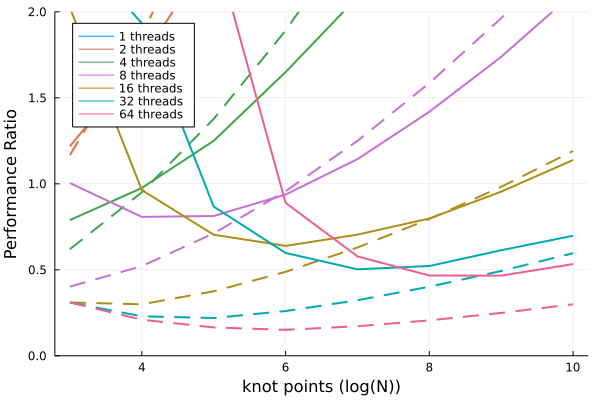
\includegraphics[width=\columnwidth]{figures/rslqr/expected_vs_actual_horizon.png}
    \includegraphics[width=\columnwidth, height=6cm]{figures/rslqr/horizon_cores_comp.tikz}
    \caption{Comparison of actual (solid lines) and theoretical (dashed lines) speedup of 
    rsLQR versus Riccati recursion for varying horizon lengths for a system with $n=14$ 
    states and $m=7$ controls. Values greater than 1 mean 
    rsLQR was faster than Riccati.}
    \label{fig:actual_vs_theoretical}
\end{figure}

\begin{figure}
    \centering 
    \includegraphics[width=\columnwidth, height=6cm]{figures/rslqr/horizon_comp.tikz}
    \caption{Comparison of solve time vs horizon length for several state-of-the-art 
    sparse matrix solvers. Parallelizable methods are followed by a number in parentheses 
    denoting the number of cores used to compute the solution. }
    \label{fig:horizon_comp}
\end{figure}

\section{Discussion} \label{sec:rslqr_conclusion}

We have demonstrated a new parallelizable algorithm for solving the sparse
linear systems that arise when solving trajectory optimization and other related
optimal-control problems.  This algorithm offers greater generality than other
LQR-based approaches, allowing straightforward adaptations to handle implicit
integration methods and constraints. With 64 parallel threads, the proposed
algorithm offers a 50\% improvement over Riccati recursion at a horizon length
of 512, while again being strictly more general in its applicability. It also
beats existing commerical parallelized sparse symmetric linear system solvers
such as HSL MA86 (by about 80\%) and Pardiso 6.0 (by about 180\%) at a horizon
length of 512, and scales much better with increased parallelism. 

Substantial areas for future work remain, such as adapting the implementation to work on
distributed-memory architectures and comparisons with distributed memory linear algebra
packages such as ScaLAPACK \cite{tennessee_ScaLAPACK_}. While our algorithm's performance was only
matched or beaten by SuiteSparse and QDLDL, these algorithms don't work on large-scale
distributed-memory architectures.  Future work may also investigate GPU or FPGA 
implementations; however, while modern GPUs have thousands of ``cores'', mapping the current
algorithm onto the SIMD-style parallelism of a GPU would require significant modification to maintain high performance due its communication and
synchronization requirements.  Future work will also investigate the performance benefits of
integrating the proposed method into nonlinear trajectory optimization methods such as 
direct collocation via sequential quadratic or convex programming. %, which includes extensions to the algorithm to allow for implicit integrators and path constraints.

While this chapter focused on leveraging parallelization across the time domain, the next
chapter considers a method for exposing parallelization across the spatial domain by 
representing the dynamics of a multi-body mechanism in maximal coordinates.

% \printbibliography


\end{document}
